% SolarMax breadboard wiring  ("look and connect")
% Built from docs/breadboard_placement.md. Every pin is a named node at an integer
% column; every wire ends on a named node or the same column's rail hole, so
% endpoints cannot drift. Compile:  pdflatex wiring_breadboard.tex
\documentclass[landscape,a4paper]{article}
\usepackage[margin=0.5cm,landscape]{geometry}
\usepackage{tikz}\usepackage{xcolor}\usepackage{adjustbox}
\usetikzlibrary{calc,backgrounds}
\pagestyle{empty}

\definecolor{net12v}{HTML}{C62828}\definecolor{netgnd}{HTML}{1565C0}
\definecolor{net5v}{HTML}{E53935}\definecolor{net3v3}{HTML}{FB8C00}
\definecolor{netmot}{HTML}{6A1B9A}\definecolor{netpwm}{HTML}{1E88E5}
\definecolor{neti2c}{HTML}{2E7D32}\definecolor{netlim}{HTML}{D81B60}
\definecolor{netanem}{HTML}{00897B}\definecolor{netana}{HTML}{6D4C41}
\definecolor{bbtan}{HTML}{F4F1E8}\definecolor{espdark}{HTML}{303030}

\tikzset{
  hole/.style={circle,draw=gray!55,fill=white,minimum size=2.4pt,inner sep=0pt},
  w/.style={line width=1.5pt},hw/.style={line width=3.2pt},
  body/.style={draw,rounded corners,fill=#1,minimum height=0.7cm,font=\scriptsize\bfseries,align=center},
  res/.style={draw,fill=yellow!30,font=\tiny,minimum height=0.42cm},
  ldr/.style={draw,fill=orange!35,font=\tiny,minimum height=0.42cm},
  lblw/.style={font=\scriptsize,text=white,inner sep=1pt},
  lbl/.style={font=\scriptsize,inner sep=1pt},
}
% y-levels
\def\yT{13.6}\def\yTG{13.1}\def\yET{8.8}\def\yEB{6.6}\def\yM{4.8}\def\yBG{1.4}\def\yB{0.8}

\begin{document}
\begin{center}{\Large\bfseries SolarMax — Breadboard Wiring}\\[1pt]
{\small Match the colors. Every blue wire ends on a blue (GND) rail. Build from \texttt{breadboard\_placement.md}.}\end{center}

\noindent\fbox{\parbox{\dimexpr\textwidth-2\fboxsep-2\fboxrule\relax}{\centering
\tikz\draw[hw,net12v](0,0)--(.55,0);\,+12V\quad
\tikz\draw[w,net5v](0,0)--(.55,0);\,+5V\quad
\tikz\draw[w,net3v3](0,0)--(.55,0);\,+3.3V\quad
\tikz\draw[w,netgnd](0,0)--(.55,0);\,GND\quad
\tikz\draw[hw,netmot](0,0)--(.55,0);\,Motor\quad
\tikz\draw[w,netpwm](0,0)--(.55,0);\,PWM/EN\quad
\tikz\draw[w,neti2c](0,0)--(.55,0);\,I\textsuperscript{2}C\quad
\tikz\draw[w,netlim](0,0)--(.55,0);\,Limit\quad
\tikz\draw[w,netanem](0,0)--(.55,0);\,Anem\quad
\tikz\draw[w,netana](0,0)--(.55,0);\,Pot/LDR}}

\vspace{3pt}
\begin{adjustbox}{max width=\textwidth,max totalheight=0.84\textheight,center}
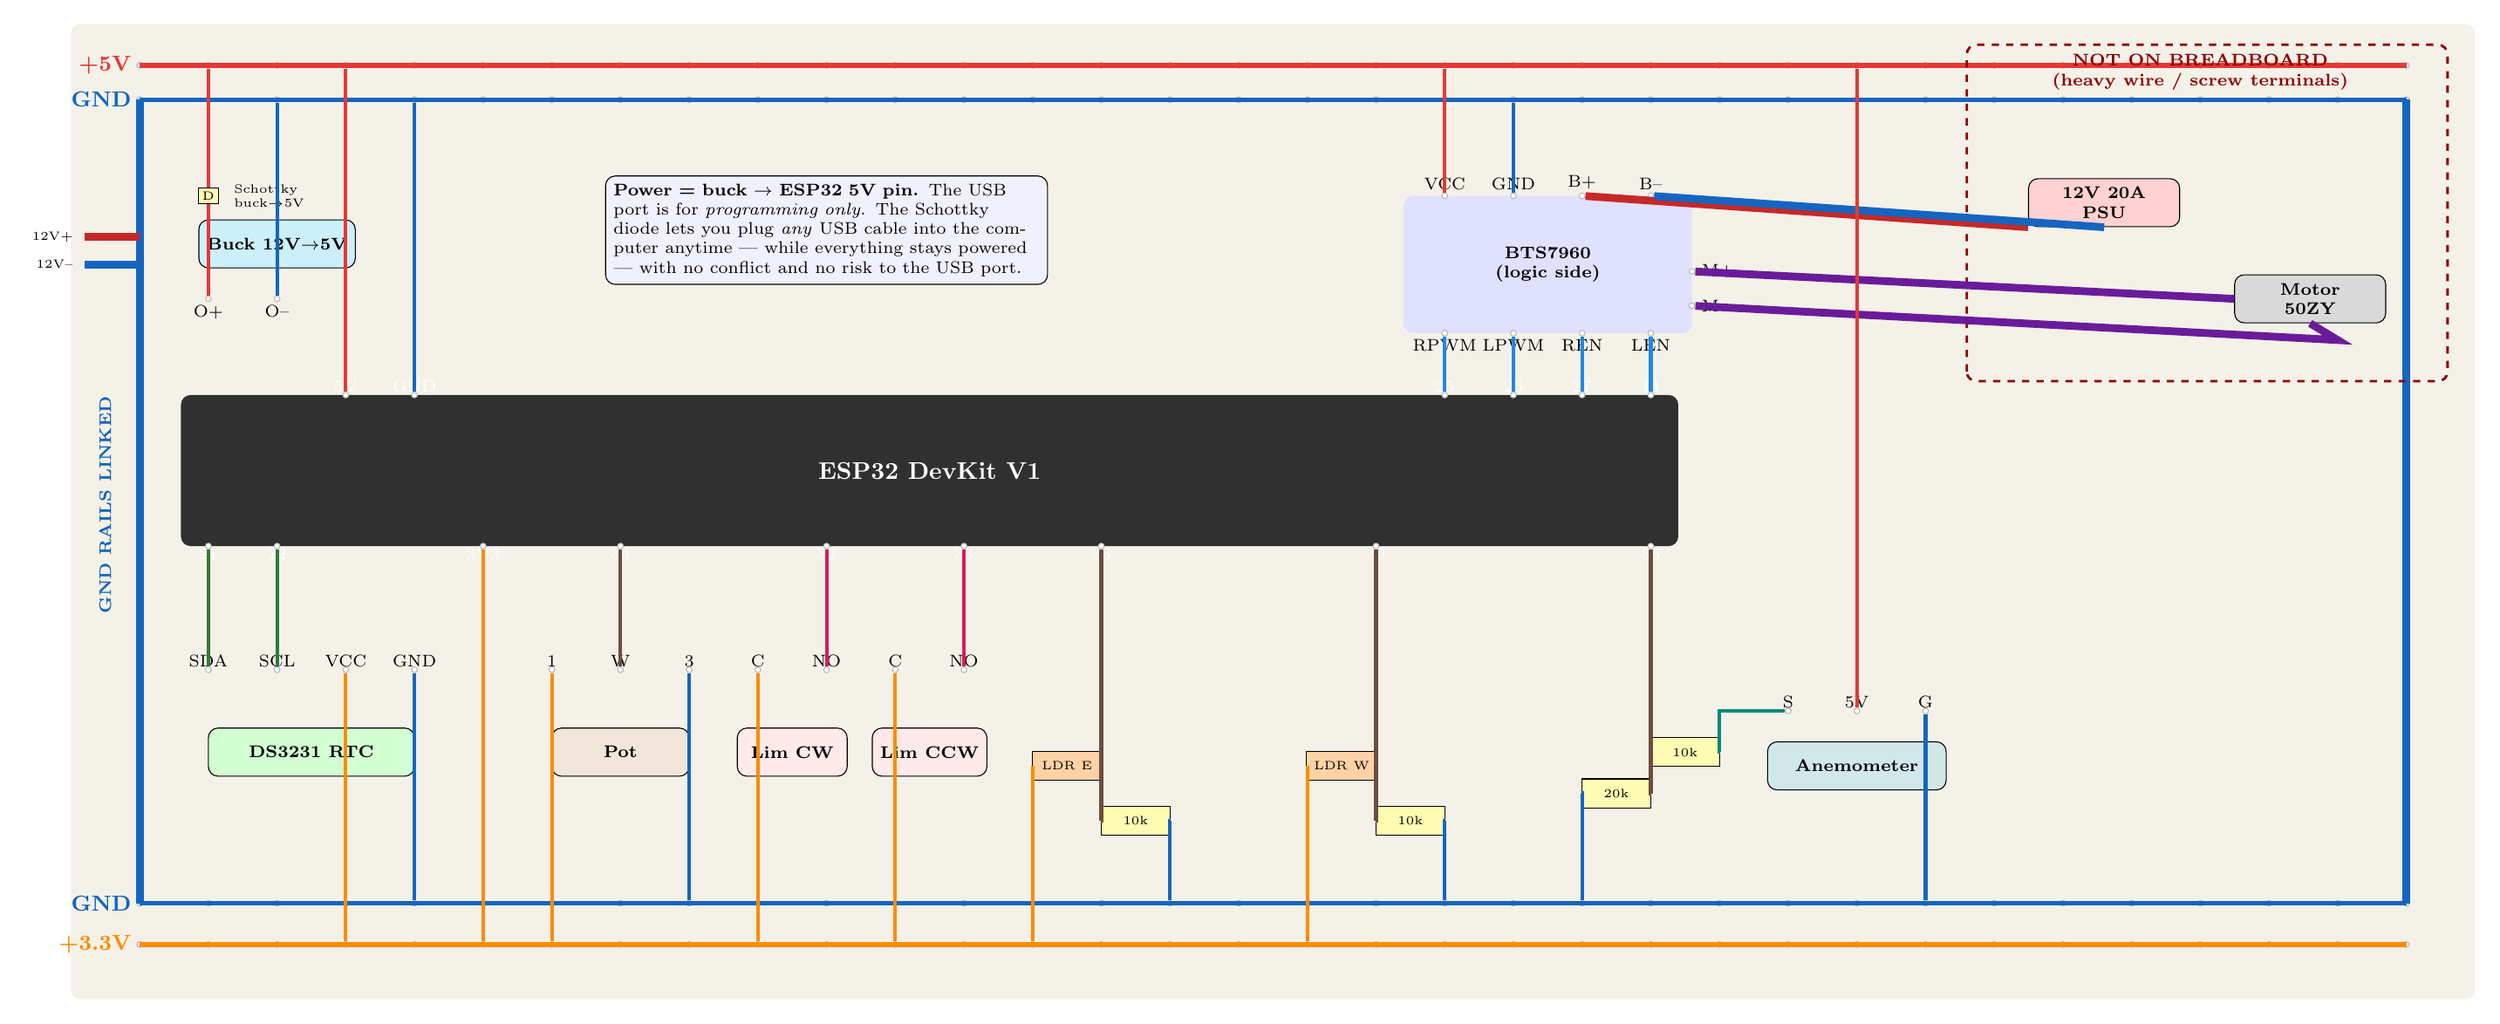
\begin{tikzpicture}[x=1cm,y=1cm]

% ===== board + rails =====
\fill[bbtan,rounded corners](0,0)rectangle(35,14.2);
\foreach \c in {1,...,34}{
  \node[hole](r5-\c)at(\c,\yT){};\node[hole](gt-\c)at(\c,\yTG){};
  \node[hole](gb-\c)at(\c,\yBG){};\node[hole](r3-\c)at(\c,\yB){};}
\draw[net5v ,line width=2pt](1,\yT)--(34,\yT);   \node[net5v ,font=\small\bfseries,left]at(1,\yT){+5V};
\draw[netgnd,line width=2pt](1,\yTG)--(34,\yTG); \node[netgnd,font=\small\bfseries,left]at(1,\yTG){GND};
\draw[netgnd,line width=2pt](1,\yBG)--(34,\yBG); \node[netgnd,font=\small\bfseries,left]at(1,\yBG){GND};
\draw[net3v3,line width=2pt](1,\yB)--(34,\yB);   \node[net3v3,font=\small\bfseries,left]at(1,\yB){+3.3V};
% common-ground ties
\draw[hw,netgnd](1,\yTG)--(1,\yBG);\draw[hw,netgnd](34,\yTG)--(34,\yBG);
\node[netgnd,font=\scriptsize\bfseries,rotate=90]at(0.5,7.2){GND RAILS LINKED};

% ===== ESP32 =====
\fill[espdark,rounded corners](1.6,\yEB)rectangle(23.4,\yET);
\node[lblw]at(12.5,7.7){\normalsize\bfseries ESP32 DevKit V1};
\foreach \nm/\c in {5V/4,GND/5,25/20,26/21,27/22,14/23}{
  \node[hole](e-\nm)at(\c,\yET){};\node[lblw,above]at(\c,\yET){\nm};}
\foreach \nm/\c in {21/2,22/3,3V3/6,34/8,32/11,33/13,36/15,39/19,35/23}{
  \node[hole](e-\nm)at(\c,\yEB){};\node[lblw,below]at(\c,\yEB){\nm};}

% ===== buck (top-left) =====
\node[body=cyan!20]at(3,11.0){Buck 12V$\to$5V};
\node[hole](buck-op)at(2,10.2){};\node[lbl,below]at(2,10.15){O+};
\node[hole](buck-om)at(3,10.2){};\node[lbl,below]at(3,10.15){O--};
\node[draw,fill=yellow!30,font=\tiny,inner sep=1.6pt](d5)at(2,11.7){D};
\node[font=\tiny,align=left,anchor=west]at(2.25,11.7){Schottky\\buck$\to$5V};
\draw[w,net5v ](buck-op)--(d5);
\draw[w,net5v ](d5)--(r5-2);
\draw[w,netgnd](buck-om)--(gt-3);
\draw[hw,net12v](1.0,11.1)--(0.2,11.1)node[left,font=\tiny,black]{12V+};
\draw[hw,netgnd](1.0,10.7)--(0.2,10.7)node[left,font=\tiny,black]{12V--};

% ===== ESP power jumpers =====
\draw[w,net5v ](e-5V)--(r5-4);
\draw[w,netgnd](e-GND)--(gt-5);
\draw[w,net3v3](e-3V3)--(r3-6);

% USB note
\node[draw,rounded corners,fill=blue!6,font=\scriptsize,align=left,text width=6.2cm]at(11,11.2)
 {\textbf{Power = buck $\to$ ESP32 5V pin.} The USB port is for \emph{programming only}.
  The Schottky diode lets you plug \emph{any} USB cable into the computer anytime — while
  everything stays powered — with no conflict and no risk to the USB port.};

% ===== off-board zone =====
\begin{scope}[on background layer]\fill[red!12,rounded corners](27.6,9.0)rectangle(34.6,13.9);\end{scope}
\draw[red!55!black,dashed,line width=1pt,rounded corners](27.6,9.0)rectangle(34.6,13.9);
\node[red!55!black,font=\scriptsize\bfseries,align=center]at(31,13.5){NOT ON BREADBOARD\\(heavy wire / screw terminals)};
\node[body=red!18,minimum width=2.2cm](psu)at(29.6,11.6){12V 20A\\PSU};
\node[body=gray!30,minimum width=2.2cm](motor)at(32.6,10.2){Motor\\50ZY};

% ===== BTS7960 (top, over 25..14) =====
\fill[blue!12,rounded corners](19.4,9.7)rectangle(23.6,11.7);
\node[font=\scriptsize\bfseries,align=center]at(21.5,10.7){BTS7960\\(logic side)};
\foreach \nm/\c in {RPWM/20,LPWM/21,REN/22,LEN/23}{
  \node[hole](b-\nm)at(\c,9.7){};\node[lbl,below]at(\c,9.65){\nm};}
\node[hole](b-vcc)at(20,11.7){};\node[lbl,above]at(20,11.75){VCC};
\node[hole](b-gnd)at(21,11.7){};\node[lbl,above]at(21,11.75){GND};
\node[hole](b-bp)at(22,11.7){};\node[lbl,above]at(22,11.75){B+};
\node[hole](b-bm)at(23,11.7){};\node[lbl,above]at(23,11.75){B--};
\node[hole](b-mp)at(23.6,10.6){};\node[lbl,right]at(23.7,10.6){M+};
\node[hole](b-mm)at(23.6,10.1){};\node[lbl,right]at(23.7,10.1){M--};
\draw[w,netpwm](b-RPWM)--(e-25);
\draw[w,netpwm](b-LPWM)--(e-26);
\draw[w,netpwm](b-REN)--(e-27);
\draw[w,netpwm](b-LEN)--(e-14);
\draw[w,net5v ](b-vcc)--(r5-20);
\draw[w,netgnd](b-gnd)--(gt-21);
\draw[hw,net12v](b-bp)--(psu.south west);
\draw[hw,netgnd](b-bm)--(psu.south);
\draw[hw,netmot](b-mp)--(motor.west);
\draw[hw,netmot](b-mm)--(33.0,9.6)--(motor.south);

% ===== RTC =====
\node[body=green!18,minimum width=3.0cm]at(3.5,3.6){DS3231 RTC};
\foreach \nm/\c in {SDA/2,SCL/3,VCC/4,GND/5}{\node[hole](rtc-\nm)at(\c,\yM){};\node[lbl,above]at(\c,\yM){\nm};}
\draw[w,neti2c](rtc-SDA)--(e-21);
\draw[w,neti2c](rtc-SCL)--(e-22);
\draw[w,net3v3](rtc-VCC)--(r3-4);
\draw[w,netgnd](rtc-GND)--(gb-5);

% ===== Pot =====
\node[body=brown!20,minimum width=2.0cm]at(8,3.6){Pot};
\foreach \nm/\c in {1/7,W/8,3/9}{\node[hole](pot-\nm)at(\c,\yM){};\node[lbl,above]at(\c,\yM){\nm};}
\draw[w,net3v3](pot-1)--(r3-7);
\draw[w,netana](pot-W)--(e-34);
\draw[w,netgnd](pot-3)--(gb-9);

% ===== Limit CW / CCW =====
\node[body=pink!35,minimum width=1.6cm]at(10.5,3.6){Lim CW};
\node[hole](lcw-C)at(10,\yM){};\node[lbl,above]at(10,\yM){C};
\node[hole](lcw-NO)at(11,\yM){};\node[lbl,above]at(11,\yM){NO};
\draw[w,net3v3](lcw-C)--(r3-10);
\draw[w,netlim](lcw-NO)--(e-32);
\node[body=pink!35,minimum width=1.6cm]at(12.5,3.6){Lim CCW};
\node[hole](lccw-C)at(12,\yM){};\node[lbl,above]at(12,\yM){C};
\node[hole](lccw-NO)at(13,\yM){};\node[lbl,above]at(13,\yM){NO};
\draw[w,net3v3](lccw-C)--(r3-12);
\draw[w,netlim](lccw-NO)--(e-33);

% ===== LDR east divider (3.3V-LDR-node15-10k-GND), node->GPIO36 =====
\node[ldr,minimum width=1.0cm](ldre)at(14.5,3.4){LDR E};
\node[res,minimum width=1.0cm](ldre10)at(15.5,2.6){10k};
\draw[w,net3v3](14,3.4)--(r3-14);                 % LDR west leg -> 3.3V
\draw[w,netana](ldre.east)--(15,3.4)--(15,2.6)--(ldre10.west);  % node col15 chain
\draw[w,netana](15,3.4)--(e-36);                  % node -> GPIO36
\draw[w,netgnd](ldre10.east)--(16,2.6)--(gb-16);  % 10k -> GND

% ===== LDR west divider, node col19 -> GPIO39 =====
\node[ldr,minimum width=1.0cm](ldrw)at(18.5,3.4){LDR W};
\node[res,minimum width=1.0cm](ldrw10)at(19.5,2.6){10k};
\draw[w,net3v3](18,3.4)--(r3-18);
\draw[w,netana](ldrw.east)--(19,3.4)--(19,2.6)--(ldrw10.west);
\draw[w,netana](19,3.4)--(e-39);
\draw[w,netgnd](ldrw10.east)--(20,2.6)--(gb-20);

% ===== Anemometer + divider (S-10k-node23-20k-GND), node->GPIO35 =====
\node[res,minimum width=1.0cm](an20)at(22.5,3.0){20k};
\node[res,minimum width=1.0cm](an10)at(23.5,3.6){10k};
\node[body=teal!18,minimum width=2.6cm](anem)at(26,3.4){Anemometer};
\node[hole](an-S)at(25,4.2){};\node[lbl,above]at(25,4.2){S};
\node[hole](an-P)at(26,4.2){};\node[lbl,above]at(26,4.2){5V};
\node[hole](an-G)at(27,4.2){};\node[lbl,above]at(27,4.2){G};
\draw[w,netgnd](an20.west)--(22,3.0)--(gb-22);    % 20k -> GND
\draw[w,netana](an20.east)--(23,3.0)--(23,3.6)--(an10.west); % node col23
\draw[w,netana](23,3.0)--(e-35);                  % node -> GPIO35
\draw[w,netanem](an10.east)--(24,3.6)--(24,4.2)--(an-S);     % 10k -> anem S
\draw[w,net5v ](an-P)--(r5-26);                   % anem 5V -> +5V rail (clear channel)
\draw[w,netgnd](an-G)--(gb-27);                   % anem G -> GND

\end{tikzpicture}
\end{adjustbox}
\end{document}
